

\section{Appendix I: Groups}
The core content of the course begins with a review of linear algebra. In the actual course, it was assumed that the student is already familiar with the notion of a vector space, as well as the notions of linear maps, eigenvalues and eigenvectors, bases, isomorphisms, and inner product spaces.

In this chapter we will provide a summary of many of the definitions we will use in the course. See standard books for more detail \cite{Aluffi2009-wb,Jacobson2009-pp,Dummit2003-rj,Roman2008-rh,Axler2015-in}. I have attempted to make this chapter thorough enough that the reader does not need to constantly look up definitions and theorems from linear algebra and abstract algebra.

The section on sets is required knowledge, although the definition of the characteristic of a field is not too important. In this course the main fields we will see are $\RR$ and $\CC$, so don't worry about knowing abstract algebraic field theory.

Much of the material on group theory I have included is also extraneous, and can be skipped. The main important thing to note is the definition of a \textbf{permutation}. Permutations are very useful tools inside and outside of group theory, and we will use them extensively. I have also included some proofs of important theorems in group theory, such as Cayley's theorem, which I believe lend some intuition to more abstract groups. However, we will not use these theorems in the course.

I have also included a short section on rings, although we will not use very many ring theoretic concepts in this course. I only included this section because when defining the Pfaffian of an antisymmetric bilinear form, we required the fact that $\ZZ[x]$ is a unique factorization domain. In general, feel free to skip the section on rings entirely.

Finally, I would like to emphasize the sections on linear algebra. Many readers will have taken a first year linear algebra course, but will not have seen some abstract definitions. If the reader wants to understand the proofs in later sections, it will be important to understand isomorphisms, linear maps, and bases. 



\subsection{Sets and Fields}

Sets allow us to essentially describe the "setting"(s) of a mathematical problem. The settings in linear algebra are vector spaces, but there are many more special kinds of sets. 

We often model new problems by combining sets in various ways. One of the simplest ways to combine two sets is called the cartesian product. The cartesian product is the collection of ordered pairs of elements from two sets. If we were to visually lay out the two sets on lines, then their Cartesian product would look like a rectangle, cut into grid squares for each pair of elements.

\begin{defn}[Cartesian Product]\index{Product!Cartesian}
Let $S_1$ and $S_2$ be any sets. Then the cartesian product $S_1 \times S_2$ of $S_1$ and $S_2$ is defined as the collection of ordered pairs of elements from $S_1$ and $S_2$. That is,
\[S_1 \times S_2 = \{(a,b) : a \in S_1 \textsf{ and } b \in S_2 \}\]

If $S$ is a set and $n$ is a positive integer, we often write,
\[S^n = \underbrace{S \times ... \times S}_{n\textsf{ times}}\]
\end{defn}

\begin{example}If $S_1 = \{1,2\}$ and $S_2 = \{3,4\}$ then $S_1\times S_2 = \{(1,3), (1,4), (2,3), (2,4)\}$.\end{example}


\begin{defn}[Set Union/Intersection] Let $A$ and $B$ be sets. Then we define the \textbf{union} of $A$ and $B$ by
\[A\cup B = \{x : x \in A \textsf{ or }x \in B\}\]
and the \textbf{intersection} of $A$ and $B$ by
\[A\cap B = \{x : x \in A \textsf{ and }x \in B\}\]  
\end{defn}
\begin{defn}[Set Complement]
    Let $A$ be a set and let $B$ be a subset of $A$. Then the \textbf{complement} of $B$ in $A$ is denoted $B^c$ and is given by
    \[B^c = \{x \in A : x \textsf{ is not in } B\}\]
\end{defn}
\begin{defn}[Set Subtraction]
Let $A$ be a set and let $B,C$ be subsets of $A$. Then we define the notation:
\[B\setminus C = B\cap C^c\]
That is, it is the set you get by removing all the common elements of $B$ and $C$ from $B$.
\end{defn}
\begin{defn}[Injective, Surjective, Bijective]\index{Injective}\index{Surjective}\index{Bijective}
    Let $f : A \to B$ be any function between sets $A$ and $B$. 
    \begin{enumerate}
    \item {
        Suppose that for all $b \in B$, there exists $a \in A$ so that $f(a)=b$. Then $f$ is called \textbf{surjective}, or "onto"
    }
    \item {
        Suppose that for all $a_1,a_2 \in A$, that $f(a_1)=f(a_2)$ if and only if $a_1=a_2$. Then $f$ is called $\textbf{injective}$, or "one-to-one".
    }
    \item {
        If $f$ is both injective and surjective, then we say $f$ is \textbf{bijective}.
    }
    \end{enumerate}
\end{defn}

\begin{defn}[Inverse Image/Fiber]\index{Fiber}
    Let $f : A \to B$ be any function between sets $A$ and $B$. Let $C\subseteq B$ be any subset of $B$. Then we define,
    \begin{equation}
        f^{-1}(C) = \{a \in A : f(a)\in C\}
    \end{equation}
    This is called the \textbf{inverse image} of $C$ under $f$. If $C = \{b\}$, then we say $f^{-1}(\{b\})$ is the \textbf{fiber} of $f$ over $b$. 
\end{defn}
The fiber of $f$ over $b$ is the set of all elements of $A$ which get mapped to $b$ by $f$.

A special kind of set that we often use to construct vector spaces is called a field. A field is a generalization of the idea of "rational numbers". A field is a set, and given some elements of this set you can perform operations which obey all the all the usual rules of arithmetic. That is, given two elements of a field, you can multiply, add, subtract, or divide them (unless the denominator is zero!)


\begin{defn}[Field]\index{Field}
A field $\FF$ is a set equipped with a notion of addition and multiplication. That is, for any two elements $x,y \in \FF$ we can add them to produce a third element $x+y \in \FF$ or we can multiply them to produce an element $xy \in \FF$. These operations must follow the field axioms, which are listed as follows.
\begin{enumerate}
\item {
Commutativity: $x+y=y+x$, $xy = yx$
}
\item {
Associativity: $x+(y+z) = (x+y)+z$, $x(yz) = (xy)z$
}
\item {
Distributivity: $x(y+z) = xy+xz$
}
\end{enumerate}
\end{defn}

One example of a field we know and love is the rational numbers $\QQ$. The rational numbers are any numbers which can be formed as the ratio of two integers. Another example is the real numbers $\RR$. The real numbers are all the numbers which can be expressed as the limit of some convergent sequence of rational numbers. We will not worry too much about how the real numbers are defined rigorously. All that matters is that you can multiply, divide, add, and subtract them. We also care about the property of the real numbers, that adding $1$ to a positive number never results in zero. This property is encapsulated in the following definition.

\begin{defn}[Characteristic]\index{Characteristic}
Let $\FF$ be a field. Then the characteristic $\textsf{char}(\FF)$ is the smallest natural number $n$ so that  $ 1+...+1 = \sum_{i=1}^n (1)= 0$. If no such natural number exists, we say $\textsf{char}(\FF) = 0$. In this course, we will primarily deal with the fields $\RR$ and $\CC$ which have characteristic zero.   
\end{defn}

\subsection{Groups}
\subsubsection{Basic Definitions}
In this course we will make some use of group theory. We are especially interested in groups of matrices, but we will also make a lot of use of permutations. This content can all be found in standard books \cite{Aluffi2009-wb,Dummit2003-rj,Jacobson2009-pp}.

\begin{defn}[Group]\index{Group}
Let $S$ be a set and suppose that there is some function $f : S \times S \to S$ which takes two elements $a$ and $b$ of $S$ and produces a third element, $f(a,b)$. We say that $S$ is a group, with operation $f$, if the function $f$ satisfies the following properties:
\begin{enumerate}
\item {
Associativity: for all $a,b,c \in S$ we have $f(a,f(b,c)) = f(f(a,b),c)$
}
\item {
Identity: There exists some element $e \in S$ so that $f(e,a) = f(a,e) = a$ for all $a \in S$.
}
\item {
Invertibilty: For all $a \in S$ there is some element $a^{-1}\in S$ so that $f(a^{-1},a) = f(a,a^{-1}) = e$.
}
\end{enumerate}
\end{defn}
\begin{defn}[Subgroup]\index{Subgroup}
    Let $G$ be a group with operation $f$ and let $H\subseteq G$. Then $H$ is a subgroup of $G$ if $H$ is a group with respect to the same operation $f$ as $G$.
\end{defn}
\begin{defn}[Order] \index{Group!Order} Let $G$ be a group. The order of $G$, denoted $|G|$, is the number of elements of $G$.
\end{defn}
\begin{example}[Trivial Group]
    The only group of order $1$ is the trivial group, $\{1\}$. This is clearly a group since $1\cdot 1 = 1$, and $1=1^{-1}$.
\end{example}
\begin{example}[Integers]\index{Group!of Integers}
The integers $\ZZ$ form a group, where the operation is $f(a,b) = a+b$. Observe that this indeed satisfies the axioms:
\begin{enumerate}
\item {
Associativity: $a+(b+c) = (a+b)+c$
}
\item {
The identity is $e=0$. We have,
$a+0 = 0+a = a$
}
\item {
The inverse element of $a$ is $-a$. We have, $a + (-a) = 0$
}
\end{enumerate}
The integers have infinite order.
\end{example}

\begin{example}
    The set of $n\times n$ invertible matrices with entries in a field $\FF$ forms a group. We often refer to this group as the \textbf{general linear group}. The symbol for it is $\GL_n(\FF)$.
\end{example}
\begin{example}
    The set of unitary matrices (i.e. matrices with the property that $U^\dagger U=\One$) forms a group, $U(n)$, called the \textbf{unitary group}. We will define this properly later.
\end{example}
\begin{example}
    The set of all orthogonal matrices forms a group called the orthogonal group, $O(n)$. We will study it in detail much later.
\end{example}
\begin{example}
    The set of unitary matrices with determinant 1 forms the special unitary group, $\SU(n)$.

    The set of orthogonal matrices with determinant 1 forms the special orthogonal group, $\SO(n)$.
\end{example}

\begin{defn}[Generating Set] \index{Group!Generating Set}Let $G$ be a group and let $S$ be a subset of $G$. We define the \textbf{group generated by $S$} to be the unique subgroup $\langle S\rangle$ of $G$ so that $\langle S\rangle$ contains $G$, and if $K$ is any other subgroup of $G$ containing $S$ we have $\langle S\rangle\subseteq K$. That is, $\langle S\rangle$ is the \textbf{smallest subgroup containing $S$}.
We call $S$ a \textbf{generating set} for $\langle S\rangle$. If $\langle S\rangle=G$ then we say $S$ \textbf{generates} $G$. If $S = \{g_1,...,g_n\}$ we usually write $\langle S\rangle = \langle g_1,...,g_n\rangle$.
\end{defn}
\begin{remark*}
    The generators of a Lie group are \textbf{not} the same concept. It is unlucky terminology.
\end{remark*}
\begin{defn}[Cyclic Group]
\index{Group!Cyclic} Let $G$ be a group. Then we say $G$ is \textbf{cyclic} if there is an element $g \in G$ so that $\langle g\rangle = G$. In other words, if $G$ is generated by one element.
\end{defn}
\begin{remark*}
    If $G=\langle g\rangle$ is cyclic then any element $k$ of $G$ can be written as $k = g^{n}$, with $n \in \ZZ$. \textbf{Reminder:} Here by ``exponentiation" we really mean repeating the group operation $n$ times! For an addition group, we actually have $k = g+...+g = ng$.
\end{remark*}
\begin{lemma}
    The integers are cyclic. We have $\ZZ = \langle 1 \rangle$.
\end{lemma}
\begin{proof}
    The proof is simply the statement that $n = 1n$ for any $n \in \ZZ$.
\end{proof}


\subsubsection{Permutations}
\begin{example}[Permutation Group]\index{Group!of Permutations}
Let $\ZZ_n = \{1,2,...,n\}$ denote the positive integers up to $n$. We define the \textbf{permutation group} (also known as the \textbf{symmetric group}) to be the following set.
\begin{equation}
    S_n = \{\sigma : \ZZ_n \to \ZZ_n : \sigma \textsf{ is bijective}\}
\end{equation}
The symmetric group has order $|S_n| = n!$.
The elements of $S_n$ are functions which simply rearrange the order of the first $n$ positive integers without removing any. The group operation is given by
\[f(\sigma,\tau) = \sigma\circ\tau,\qquad \sigma\in S_n,\tau\in S_n\]
Which is just the composition of the two permutations. This satisfies the group axioms:
\begin{enumerate}
\item {
Associative: $\sigma\circ(\tau\circ \chi)(1,...,n) = \sigma(\tau(\chi(1,...,n))) = (\sigma\circ\tau)\circ\chi(1,...,n)$
}
\item {
Identity: Let $e(1,...,n) = (1,...,n)$. Then $\sigma \circ e = e\circ \sigma = \sigma$.
}
\item {
Invertibility: Since $\sigma$ is bijective, we have $\sigma \circ \sigma^{-1} = \sigma^{-1}\circ\sigma = e$.
}
\end{enumerate}
A permutation map is primarily defined as a function from $\ZZ_n$ to $\ZZ_n$. But we also often use them to act on an ordered list of symbols $(v_1,...,v_n)$ to get a new list $\sigma(v_1,...,v_n) =(v_{\sigma(1)},...,v_{\sigma(n)})$ which is the same list, just reordered.
\end{example}
\begin{example}[Transposition]\index{Transposition}
Consider the permutation which swaps the order of the first two inputs:
\[\sigma_{12}(v_1,v_2,v_3,...,v_n) = (v_2,v_1,v_3,...,v_n)\]
A permutation which does nothing but swap two symbols is called a \textbf{transposition}. Observe that if we applied $\sigma_{12}$ twice, we would get,
\[\sigma_{12}^2(v_1,v_2,v_3,...,v_n) = \sigma_{12}(v_2,v_1,v_3,...,v_n) = (v_1,v_2,v_3,...,v_n)\]
So $\sigma_{12}^{-1} = \sigma_{12}$. In general, any transposition is its own inverse.
\end{example}
\begin{figure}[h]
    \centering
    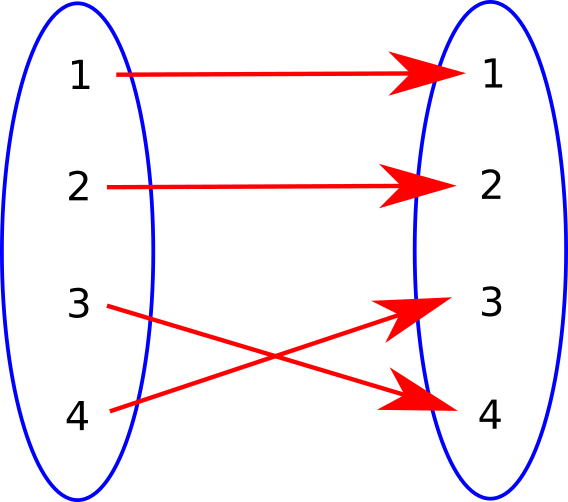
\includegraphics[width=0.5\linewidth]{transposition.png}
    \caption{Diagram of an example transposition.}
    \label{fig:transposition}
\end{figure}

\begin{defn}\index{Parity}
    Let $S_n$ denote the permutation group on $\{1,...,n\}$. We say that $\sigma \in S_n$ is an \textbf{even permutation} if it can be reproduced by an even number of transpositions. It is called an \textbf{odd permutation} if it can be reproduced by an odd number of transpositions.
    
    The \textbf{parity} $\sgn(\sigma)$ of a permutation is defined as follows.
    \[\sgn(\sigma) = \begin{cases}1 &\textsf{if } \sigma \textsf{ is even}\\
    -1 & \textsf{if } \sigma \textsf{ is odd}\end{cases}\]
\end{defn}
\begin{example}
    Any transposition is an odd permutation by definition.
\end{example}
\begin{example}
Let $n=3$. The permutation taking $(1,2,3)$ to $(2,3,1)$ can be achieved by swapping 1 and 3, then swapping 2 and 3. It is therefore an even permutation.
\end{example}
\begin{thm}[Decomposition of Permutations]
    Let $\sigma\in S_n$ be a permutation. Then there exists a finite list $\{\tau_1,...,\tau_N\}$ of transpositions so that $\sigma = \tau_1\circ...\circ \tau_N$. 

    In other words, if $T_n$ is the set of all transpositions in $S_n$ then $S_n = \langle T_n\rangle$.
\end{thm}
\begin{thm}
Parity satisfies the property that $\sgn(\sigma\circ\tau) = \sgn(\sigma)\sgn(\tau)$.
\end{thm}
\begin{cor}
    The parity of $\sigma$ can also be written as,
    \[\sgn(\sigma) = \begin{cases}1 &\textsf{if } \sigma \textsf{ is the product of an even number of transpositions}\\
    -1 & \textsf{if } \sigma \textsf{ is the product of an odd number of transpositions}\end{cases}\]
\end{cor}

\subsubsection{Group Homomorphisms}

\begin{defn}[Group Homomorphism]\index{Homomorphism!Group}
Let $G$ and $H$ be groups. Let $\phi : G \to H$ be a function.

Denote the group operation of $G$ by $f_G(g_1,g_2)$ and the group operation of $H$ by $f_H(h_1,h_2)$. We say $\phi$ is a \textbf{group homomorphism} (or just a \textbf{homomorphism}) if the following equation holds,
\[\phi(f_G(g_1,g_2)) = f_H(\phi(g_1),\phi(g_2))\]
\end{defn}
\begin{defn}[Kernel and Image]\index{Kernel!of Group Homomorphism}\index{Image!of Group Homomorphism}
    Let $\phi : G \to H$ be a group homomorphism.
    
    The image of $\phi$ is defined by $\image(\phi) = \{\phi(x): x\in G\}$. It is a subgroup of $H$.

    The kernel of $\phi$ is defined by $\ker(\phi) = \{x\in G: \phi(x)=e\}$. It is a subgroup of $G$.
\end{defn}
\begin{remark*}
    The kernel consists of anything getting mapped to the identity.

    The image is the set of all outputs.
\end{remark*}
\begin{thm}
    Consider the group $G = \{-1,1\}$, where the group operation is $f_G(a,b) = ab$. The map $\sgn : S_n \to G$ is a group homomorphism.
\end{thm}
\begin{proof}
    As we saw earlier, $\sgn(\sigma\circ\tau) = \sgn(\sigma)\sgn(\tau)$.
\end{proof}
\begin{defn}[Alternating Group]\index{Group!Alternating}
    The kernel of the map $\sgn : S_n \to G$ is denoted $\ker (\sgn) = A_n$, and is called the alternating group. It consists of all even permutations in $S_n$. It has order $|A_n| = n!/2$.
\end{defn}


\begin{defn}[Group Isomorphism]\index{Isomorphism!of Groups}
Let $G$ and $H$ be groups, and let $\phi : G \to H$ be a group homomorphism. If $\phi$ is bijective, we say it is a \textbf{group isomorphism}. Group isomorphism is an equivalence relation. 
\end{defn}

\begin{lemma}
    Suppose $\phi : G \to H$ is an injective group homomorphism. Then $\phi$ is an isomorphism between $G$ and $\image(\phi)$
\end{lemma}
\begin{proof}
    Let $y \in \image(\phi)$. Then by definition, there is an element $x$ of $G$ with $\phi(x)=y$. Therefore $\phi$ is surjective onto $\image(\phi)$. This completes the proof.
\end{proof}
\begin{lemma}
    Any two cyclic groups $G,H$ of order $|G|=|H|$ are isomorphic.
\end{lemma}
\begin{proof}
    Recall that $G = \langle g\rangle$ and $H = \langle h \rangle$.
    
    First we show that there is a unique homomorphism $\phi: G\to H$ so that $\phi(g) = h$. Suppose $\phi_1$ and $\phi_2$ are homomorphisms and that $\phi_1(g)=\phi_2(g)=h$. Then $\phi_1(g)^n = \phi_1(g^n)$ and $\phi_2(g)^n = \phi_2(g^n)$. So $\phi_1(g^n) = h^n=\phi_2(g^n)$ for all $n$. Since every element of $G$ is of the form $g^n$, we see that $\phi_1(x)=\phi_2(x)$ for all $x\in G$. Thus $\phi$ is unique.

    Now we show that it is surjective. Suppose $k \in H$. Then for some $|n|\leq |G|=|H|$, we have $k = h^n = \phi(g)^n = \phi(g^n)$.

    Finally, we show it is injective. Suppose $\phi(x) = e$. Then $\phi(x)k=k$ for all $k\in H$. So for some $n$ we have $\phi(x)h^n = h^n$, so $\phi(xg^n) = h^n$. Since $x \in G$ we have $x = g^q$ for some $q$, so $\phi(g^{q+n}) = h^n$. But $\phi(g^{q+n}) = h^{q+n}$. So we must have $q = a|G|$ for some $a \in \ZZ$. But $|G| = |H|$, so $g^{n+q} = g^n$ and $h^{n+q} = h^n$. This completes the proof.
\end{proof}
\begin{lemma}
    Let $G=\langle g\rangle$ be cyclic and finite. Then $g^{|G|} = e$. Furthermore, $g^{a+|G|k} = g^a$ for all $k\in\ZZ$.
\end{lemma}
\begin{remark*}
    This is why we call it a cyclic group.
\end{remark*}
\begin{proof}
Let $\ell$ be the smallest integer so that $g^\ell = e$. We can always write $k = \ell q+r$ for some remainder $r$, so $g^{\ell q+r} = g^{\ell q}g^r = e$. But $g^{\ell q} = (g^\ell)^q = e^q = e$. So $r=0$. Therefore if $g^k = e$ we must have $k = \ell q$ for some $q$.
We also have that for all $0< k\leq \ell-1$, $g^{-k} = g^a$ for some $a$. Since $g^\ell = e$, this means that $g^{\ell-k} = g^{-k}$. Since $0\leq \ell-k\leq \ell-1$ we have $a=\ell-k$. So $g^{-k} = g^{\ell-k}$.

Finally, observe that since $g^{-k} = g^{\ell - k}$ for all $k$, we have the following distinct elements of $G$: $\{e, g^1,g^2,...,g^{\ell-1}\}$. Thus $|G| = \ell$ and $g^{|G|} = e$ as required.
\end{proof}


\subsubsection{Quotient Groups and the First Isomorphism Theorem}
\begin{defn}[Coset of $h$] \index{Coset} Let $G$ be a group and let $h \in G$. Then the set $hG = \{hg : g \in G\}$ is called the right coset of $h$. The set $Gh = \{gh : g \in G\}$ is called the left coset of $h$.
\end{defn}
\begin{defn}[Coset of $H$] Let $G$ be a group and let $H$ be a subgroup of $G$. Then we define the left coset of $H$ to be $GH = \{gh : g\in G, h\in H\}$ and the right coset to be $HG = \{hg : g\in G, h \in H\}$.
\end{defn}
\begin{remark*}
    In general, we write $aHb = \{ahb : h \in H\}$. Similarly, $AHB=\{ahb : h \in H, a\in A, b\in B\}$.
\end{remark*}
\begin{defn}[Normal Subgroup]\index{Subgroup!Normal}
    Let $G$ be a group and let $H$ be a subgroup. Then we say $H$ is \textbf{normal} if $g^{-1} H g = H$ for all $g\in G$.
\end{defn}
\begin{thm}
    The following are equivalent.
    \begin{enumerate}
    \item {
    $H$ is normal.
    }
    \item {
    $g^{-1} H g = H$ for all $g \in G$.
    }
    \item {
    $gH = Hg$ for all $g \in G$.
    }
    \item {
    If $x \in aH$ and $y \in bH$ then $xy \in (ab)H$.
    }
    \item {
    For all $x,y \in G$ we have $(xH)(yH) = (xy)H$.
    }
    \item {
    There exists a group $K$ and a group homomorphism $\phi : G \to K$ with $\ker(\phi) = H$.
    }
    \end{enumerate}
\end{thm}
\begin{remark*}
    In other words, normal subgroups are just all the possible kernels of different maps out of $G$.
\end{remark*}
\begin{defn}[Quotient Group]\index{Group!Quotient}\index{Quotient!of Groups}
Let $G$ be a group and let $H$ be a normal subgroup of $G$. Then we define the quotient of $G$ by $H$ to be the collection of all cosets of $H$.
\begin{equation}G/H = \{gH : g \in G\}
\end{equation}
The set $G/H$ of all cosets of $H$ forms a group with the same operation as $G$, since $(aH)(bH) = (ab)H$.
\end{defn}
\begin{thm}[First Isomorphism Theorem/Noether's First Theorem]\index{Theorem!First Isomorphism Theorem (for Groups)}
    Let $\phi : G \to K$ be a surjective group homomorphism. Then $K$ is isomorphic to $G/\ker(\phi)$.
\end{thm}
\begin{proof}
    Let $g\ker(\phi) \in G/\ker(\phi)$. Then for any $gh \in g\ker(\phi)$ we have \[\phi(gh) = \phi(g)\phi(h) = \phi(g)e = \phi(g)\]

    Therefore, the map $\tilde{\phi} : G/\ker(\phi) \to K$, given by $\tilde{\phi}(g\ker(\phi)) = \phi(g)$, is well defined.
    
    As we can see, $\tilde{\phi}(g\ker(\phi)) = e$ if and only if $\phi(g) = e$, which means $\tilde{\phi}$ is injective. This completes the proof
\end{proof}
\begin{cor}
    $G/\ker(\phi)$ is isomorphic to $\image(\phi)$.
\end{cor}
\begin{thm}[Lagrange's Theorem]\index{Theorem!Lagrange's Theorem}
    If $H$ is a subgroup of $G$ then $|G|/|H|$ is an integer. In other words, the order of $H$ divides the order of $G$.
\end{thm}
\begin{proof}
    Consider the collection of left-cosets of $H$. 
    
    Suppose $x=gh_1 \in gH$. Then $x \in kH$ if and only if $x = kh_2$ for some $h_2\in H$, which means $gh_1 = kh_2$, or in other words, $gh_1h_2^{-1}=k$. 
    
    Since $h_1h_2^{-1} \in H$, it follows that $gH = kH$. Thus, two left cosets must be either equal or entirely disjoint. 
    
    Additionally, every left coset of $H$ is the same size since $|gH| = |H|$ for all $g$. Since there are an integer number of left cosets, it follows that $n|H|=|G|$, where $n$ is the number of left cosets of $H$.
    
    The number $n$ is called the \textbf{index}\index{Index!of Subgroup} of $H$ in $G$, and we often write it as $n = [G:H]$ so that $|H|[G:H] = |G|$.
\end{proof}

\subsubsection{Group Actions and Cayley's Theorem}
\begin{defn}[Group Action] \index{Group!Action} Let $S$ be a set and let $G$ be a group. Then a (left) \textbf{group action} is a function $A : G\times S \to S$, with the following properties:
\begin{enumerate}
\item {
Compatibility: $A(gh,s) = A(g,A(h,s))$.
}
\item {
Identity: $A(e,s) = s$.
}
\end{enumerate}
Notationally, we often write $A(g,s) = g\cdot s$ as long as this can't be confused with some other operation.
\end{defn}
\begin{defn}[Transitive Action]
\index{Group!Action!Transitive}
    A group action $A: G\times S \to S$ is called transitive, if for all $x,y \in S$ there exists some $g$ with $A(g,x) = y$.
\end{defn}
\begin{thm}[Cayley's Theorem] Any finite group $G$ is isomorphic to a subgroup $H$ of $S_n$, for some $n \in \NN$.
\end{thm}
\begin{proof}
Let $k = |G|$ be the order of $G$. Consider the left group-action of $G$ on itself, $A : G \times G\to G$ given by $A(g,h) = gh$. 

We can see that the action is invertible, since $A(g^{-1},g) =A(g,g^{-1}) = e$. 

We can also see that $A$ is transitive, since if $x,y \in G$ we have $x^{-1}y\in G$, so we can simply take $A(x,x^{-1}y) = y$. 

Therefore, for each $g \in G$ we have an invertible function $A_g : G \to G$ defined by $A_g(h) = A(g,h)$.

Since $|G|=k$, each function $A_g$ simply permutes the $k$ elements of $G$ around. Therefore we have a mapping $\tilde{A} : G \to S_k$ given by $\tilde{A}(g) = A_g$. 

We also have \[\tilde{A}(g)\tilde{A}(h)(x) = ghx = \tilde{A}(gh)(x)\]

Therefore $\tilde{A}$ is a homomorphism, and $\image(\tilde{A})$ is a subgroup of $S_k$. 

Since $\tilde{A}(g)(h) = gh = e$ iff $g = h^{-1}$, it also follows that $\tilde{A}$ is injective, and is hence an isomorphism between $G$ and $\image(\tilde{A})$ as required.
\end{proof}

\subsection{Rings}
We will only review a few definitions for rings.
\begin{defn}[Ring]\index{Ring}
Let $R$ be a commutative group. That is, there exists an operation $+ : R \times R \to R$ which is associative, commutative, invertible, and has an identity $0$. Suppose there is another operation, $\cdot : R\times R \to R$, which satisfies the following properties,
\begin{enumerate}
\item {Associative: $a\cdot(b\cdot c) = (a\cdot b)\cdot c$}
\item {Distributive: $a\cdot(b+c)=a\cdot b + a\cdot c$ and $(b+c)\cdot a = b\cdot a + c\cdot a$}
\item {Identity: There exists $1\in R$ so that $1\cdot a = a\cdot 1 = a$ for all $a$.}
\end{enumerate}
Then we say that the data $(R,+,\cdot)$ forms a \textbf{ring}. For short, we just call $R$ a ring and we usually write $a\cdot b = ab$.
\end{defn}
\begin{defn}[Ideal]
    A \textbf{ring ideal} is a subset $I\subseteq R$ with the following properties.
    \begin{enumerate}
    \item {$I$ is a subgroup of $R$ with respect to addition.}
    \item {For all $a \in R$, $b\in I$, we have $ab \in I$}
    \end{enumerate}
\end{defn}
\begin{defn}[Generating Set of Ideal]
    The \textbf{ideal generated by} a subset $S$ is defined to be the smallest ideal containing $S$. We denote it $(S)$. For $S=\{a_1,...,a_n\}$ we let $(S) = (a_1,...,a_n)$.  
\end{defn}
\begin{example}
    $\ZZ,\QQ,\RR,\CC$ are all rings.
\end{example}
\begin{example}
    Let $R$ be a ring. Let $R[x]$ denote the set of all polynomials whose coefficients are elements of $R$. Then $R[x]$ is also a ring.
\end{example}
\begin{defn}[Coset of Ideal]\index{Coset!Ideal}
    Let $I$ be an ideal in $R$. Then we define the cosets of $I$ to be the sets of the form $a+I$, $a\in R$. This is exactly the same as the construction for subgroups.
\end{defn}
\begin{defn}[Quotient Ring]
    Let $I$ be an ideal in $R$. Then we define $R/I$ to be the set of all cosets of $I$. This forms a ring.
\end{defn}
\begin{example}
    Let $R = \RR$ and consider the set of all real polynomials $\RR[x]$. Observe that $x^2 +1$ has no roots in $\RR$, which means it can not be factored. Let $(x^2+1)$ be the ideal generated by this polynomial.
    
    The quotient, $\RR[x]/(x^2+1)$, consists of all objects of the form $f(x)+I$, and two polynomials in $\RR[x]/(x^2+1)$ are said to be equivalent if they differ by a polynomial of the form $h(x)(x^2+1)$.

    Let $\phi : \RR[x]/(x^2+1)\to \CC$ be defined as follows. $\phi([f]) = f(i)$. Observe that since $i^2-1=0$, this does not depend on the choice of representative for $[f]=f+I$. Additionally, \[\phi([f]+[g])= f(i)+g(i) = \phi([f])+\phi([g])\]
    and \[\phi([fg]) = f(i)g(i) = \phi([f])\phi([g])\]
    So $\phi$ is a ring homomorphism.

    Suppose $f$ is a degree $k$ polynomial. Then it is of the form $f(x) = a_k x^k + ... + a_2 x^2 + a_1 x + a_0$. Then we can rearrange this as follows. 
    \begin{align*}f(x) +I&= a_kx^{k-2}(x^2 -1 +1) + ... + a_2(x^2-1+1) + a_1 x + a_0 + I\\
    &= (a_k x^{k-2}+...+a_2)(x^2+1) - (a_k x^{k-2} + ... + a_2) + a_1 x + a_0+I\\
    &=  - (a_k x^{k-2} + ... + a_2) + a_1 x + a_0 + I\\
    &= -(a_k x^{k-4}(x^2-1+1)+...+a_4(x^2-1+1)) + (a_1-a_3)x+(a_0-a_2) + I\\
    &=...\\
    &= (a_1\pm a_3\pm ...\pm a_{p})x+(a_0\pm a_2\pm ...\pm a_q) + I
    \end{align*}   
    Where $p$ is the largest even number less than or equal to $k$, and $q$ is the largest odd number less than or equal to $k$. Therefore we see that for any $f +I\in \RR[x]/(x^2+1)$ we can reduce $f$ to a first order polynomial. Since the coefficients $a_i$ can be chosen however we want, this means that for any $a,b\in \RR$ there is a polynomial $f$ so that $\phi([f]) = a+bi$. So $\phi$ is surjective.

    Finally, let $\phi^{-1}(a+bi) = a+bx$. Then since any $[f]$ has a first order representative, $\phi^{-1}$ is surjective. 
    
    Therefore $\phi$ is a ring isomorphism.

    Thus we have shown that $\CC$ is isomorphic to $\RR[x]/(x^2+1)$.
\end{example}
\begin{remark*}
    This is one way of defining the complex numbers. In this course we will study another definition in depth, called the Cayley-Dickson construction, which defines $\CC$ as a vector algebra over $\RR$.
\end{remark*}
\begin{defn}[Field (alternative definition)]\index{Field!Definition using rings}
    Let $R$ be a ring. Then if for all $0\neq a \in R$ there exists $a^{-1} \in R$ so that $a\cdot a^{-1} = a^{-1} \cdot a=1$, we say $R$ is a \textbf{field}.
\end{defn}

\section{Appendix II: Linear Algebra}
\subsection{Vector Spaces}
\subsubsection{Basic Definitions}
This content can all be found in standard books \cite{Axler2015-in,Roman2008-rh}
\begin{defn}[Vector Space]\index{Vector!Space}
A vector space is defined by the data of a set $V$, along with a field $\FF$ called the set of scalars. The set $V$ is equipped with a notion of addition. That is, for any two vectors $v$ and $w$ in $V$, we can add them to produce a third vector $v+w$.

In addition to this notion of vector addition, we also have a notion of scalar multiplication. That is, the vectors $v \in V$ can be scaled by an element $a$ of $\FF$ to produce a new vector $av \in V$. 

These two operations must follow the vector space axioms.
\begin{enumerate}
\item {
Commutativity: if $v,w \in V$ then $v + w = w+v$
}
\item {
Associativity: if $a,b \in \FF$ and $v \in V$, we have $a(bv) = (ab)v$
}
\item {
Distributivity: if $a \in \FF$ and $v,w \in V$ we have $a(v+w)=av+aw$.
}
\end{enumerate}
\end{defn}
\begin{remark*}
    If we replace the field $\FF$ in the above definition with an arbitrary ring $R$, then we get something called a \textbf{module} instead of a vector space.\index{Module}
\end{remark*}
\begin{defn}[Linear Subspace]\index{Linear!Subspace} Let $V$ be a vector space. A linear subspace is a subset $U \subseteq V$ which is also a vector space, with the same underlying field, scalar multiplication, and addition operations.
\end{defn}

\begin{example}
There are a great many examples of vector spaces. I will list just a few kinds of vector spaces we will encounter.

\begin{enumerate}
\item {
Vector spaces of the form $\FF^n$, such as $\RR^n$ or $\CC^n$. These are formed by taking the Cartesian product of a field with itself $n$ times. The addition operation is defined by $(a_1,...,a_n) + (b_1,...,b_n) = (a_1+b_1,...,a_n+b_n)$.
}
\item {
Vector spaces of functions. For example, $C_0(\RR)$ denotes the set of continuous functions from $\RR$ to $\RR$. This set is a vector space since we know that two continuous functions can be added to produce a third continuous function. They can also be scaled by real numbers, and the result will still be continuous.
}
\item {
Vector spaces formed by combining two vector spaces in some nice way. For example, if $V$ and $W$ are vector spaces we could form the direct sum of $V$ and $W$. The direct sum, denoted $V \oplus W$, is the set of all linear combinations of elements of $V$ and $W$.
}
\end{enumerate}
\end{example}
\begin{defn}[Span]\index{Span}
Let $V$ be a vector space over $\FF$. Let $v_1,...,v_n$ be a collection of vectors in $V$. We define
\begin{equation}
    \Span(\{v_1,...,v_n\}) = \left\{\sum_{i=1}^n a_i v_i : a_i \in \FF\right\}
\end{equation}
\end{defn}

\begin{defn}[Direct Sum]\index{Direct!Sum} Let $V$ and $W$ be vector spaces. The direct sum of $V$ and $W$ is the vector space 
\begin{equation}V\oplus W = \{v+w: v \in V, w \in W\} = \textsf{span}(V\cup W)\end{equation}
For a list of $k$ vector spaces $V_1,...,V_k$ we write,
\begin{equation}
    V_1\oplus...\oplus V_k = \bigoplus_{i=1}^k V_i
\end{equation}
\end{defn}

\begin{example}
    Let $V$ and $W$ be vector spaces. Then their Cartesian product $V \times W$ is a vector space.
\end{example}
\begin{proof}
    Consider $a \in \FF$, $(v_1,w_1) \in V \times W$ and $(v_2,w_2)\in V\times W$. Then we define addition and scalar multiplication according to the rule $(v_1,w_1)+a(v_2,w_2) = (v_1+av_2,w_1+aw_2)$. As we can see, this is an element of $V \times W$. We can verify each of the vector space axioms as well:
    \begin{enumerate}
    \item {
    $(v_1,w_1) + (v_2,w_2) = (v_1+v_2,w_1+w_2) = (v_2+v_1,w_2+w_1) = (v_2,w_2)+(v_1,w_1)$
    }
    \item {
    $a(b(v,w)) = a(bv,bw) = ((ab)v,(ab)w) = (ab)(v,w)$
    }
    \item {
    \begin{align*}
    a((v_1,w_1)+(v_2,w_2)) &= a(v_1+v_2,w_1+w_2)\\
    &= (av_1+av_2,aw_1+aw_2)\\
    &= (av_1,aw_1) + (aw_1,aw_2)\\
    &= a(v_1,w_1)+a(v_2,w_2)
    \end{align*}
    }
    \end{enumerate}
\end{proof}

An important property of vectors is linear independence.
\begin{defn}[Linearly Independent]\index{Linear!Independence}
    Let $V$ be a vector space over $\FF$. Then a collection of $n$ nonzero vectors $v_1,...,v_n$ are called linearly independent if the following property holds.
    
    Whenever $a_1,...,a_n \in \FF$ then $a_1v_1+...+a_nv_n = 0$ if and only if $a_1=...=a_n=0$. 
\end{defn}
\begin{example}
    Consider $V = \RR^3$. Then the vectors $e_1=(1,0,0)$, $e_2=(0,1,0)$, and $e_3=(0,0,1)$ are linearly independent.
\end{example}
\begin{proof}
Suppose $a_1e_1+a_2e_2+a_3e_3=0$. Observe that $a_1e_1+a_2e_2+a_3e_3 = (a_1,a_2,a_3)$. Since $(a_1,a_2,a_3)=(0,0,0)$, we must have $a_1=0,a_2=0,a_3=0$. Therefore $e_1,e_2,e_3$ must be linearly independent.
\end{proof}

\begin{defn}[Dimension]\index{Vector Space!Dimension}
    Let $V$ be a vector space over $\FF$. The dimension $\dim V$ is the largest possible number $n$ with the property that there exists a set of linearly independent vectors of size $n$.
\end{defn}

\begin{defn}[Basis]
    Let $V$ be a vector space and let $B$ be a set of linearly independent vectors such that $V = \textsf{span}(B)$. We say that $B$ is a basis for $V$.
\end{defn}
\begin{thm}
    Let $V$ be a finite dimensional vector space. Then every basis for $V$ has $\dim V$ elements. Furthermore, if $B$ is a linearly independent subset of $V$ of size $\dim V$, then $B$ is a basis for $V$.
\end{thm}
\begin{thm}
    Let $V$ be a vector space and let $W$ be a subspace of $V$. Then if $\dim W = \dim V$ we have $W=V$.
\end{thm}
\begin{proof}
    Let $\{e_1,...,e_n\}$ be a basis for $W$. Then if $V$ is $n$-dimensional, $e_1,...,e_n$ must also be a basis for $V$. Therefore $V = \textsf{span}\{e_1,...,e_n\} = W$.
\end{proof}

\begin{thm}
    Let $V$ be a vector space and let $U,W$ be subspaces of $V$. Then their intersection $U\cap W$ is a vector space, and $U\cap W = \{0\}$ if and only if $U$ and $W$ are linearly independent subspaces.
\end{thm}
\begin{remark*}
    The union of two vector subspaces is \textbf{not necessarily} a vector space.
\end{remark*}
A very special kind of vector space merits its own definition. Vector algebras are vector spaces with a notion of vector multiplication. 

\begin{defn}[Algebra]\index{Vector!Algebra}\index{Algebra} An \textbf{algebra} is a vector space equipped with a notion of vector multiplication. That is, for any two vectors $v,w \in V$ we can multiply them to produce a third vector, $v \times w$. This operation is not required to be commutative, but must satisfy the following axioms:
\begin{enumerate}
\item {
Distributivity: for all $u,v,w \in V$ we have $u\times(v+w) = u\times v + u\times w$
}
\item {
Scaling rule: for all $a \in \FF$, and $u,v\in V$, we have $a(v\times w) = (av) \times w = v\times (aw)$
}
\end{enumerate}
If in addition the algebra satisfies $u\times (v\times w) = (u\times v) \times w$, we say $A$ is an \textbf{associative algebra}.
\end{defn}
\begin{remark*}
    We call this type of vector space an ``algebra" because it has all of the tools required to do algebra: multiplication and addition.
\end{remark*}
\begin{defn}
    Let $V$ be an algebra and let $W$ be a vector subspace of $V$. Then $W$ is said to be a subalgebra of $V$ if for all $a,b\in W$ we have $ab\in W$ and $ba \in W$.\index{Subalgebra}\index{Algebra!Subalgebra}
\end{defn}
\begin{example}[Examples of Algebras]
The following are a few examples of algebras.
\begin{enumerate}
\item {
Matrix algebras.\index{Matrix!Algebra} The set $M_{nn}(\RR)$ of n by n matrices forms an algebra, where the "vector multiplication" is really just matrix multiplication. Note that this is not commutative! Many algebras are isomorphic to matrix algebras (this isomorphism is called a faithful representation).
}
\item {
The set of continuous functions, $C_0(\RR)$, has the property that if $f$ and $g$ are continuous, then their composition, $f \circ g$, is continuous. Therefore $C_0(\RR)$ is a vector algebra, where the ``multiplication" is composition. Note that this is not commutative! $f\circ g \neq g \circ f$.
}
\item {
The spaces $\RR^1$, $\RR^3$, and $\RR^7$ all have a special operation defined on them called the cross product. This is denoted $v \times w$, and it also has the property that $v \times w = -w \times v$. Therefore, $\RR, \RR^3$ and $\RR^7$ are algebras when equipped with the cross product.
}
\end{enumerate}
\end{example}
\begin{example}[Non-example of an Algebra]
The set $\GL_n(\RR)$ of invertible $n\times n$ matrices is \textbf{not} an algebra since not every linear combination of invertible matrices is invertible. It is closed under matrix multiplication but not addition. For instance, if $M\in \GL_n(\RR)$ then $M-M=0\not\in \GL_n(\RR)$ since the zero matrix is not invertible.

\end{example}
\subsubsection{Maps Between Vector Spaces}

The vast majority of the time we are only going to be interested in maps between vector spaces which don't interfere with the laws of arithmetic. That is, you should be able to scalar multiply or add vectors before applying a map, and get the same thing if you were to apply the map and then add/scale the result.

Maps with this property are called homomorphisms, or "structure preserving maps". In the case where the operations we would like to preserve are vector space operations, these maps are what we call "linear".

\begin{defn}[Linear Map] \index{Linear!Map} Let $V$ and $W$ be vector spaces over $\FF$. Then a map $T : V \to W$ is called linear if for all $a \in \FF$ and $u,v \in V$, we have $T(au+v) = aT(u)+T(v)$. If $W=V$ we say $T$ is a \textbf{linear operator}.\index{Linear!Operator}
\end{defn}
\begin{defn}[Space of Linear Maps]
    The set of all linear maps from $V$ to $W$ is denoted $L(V,W)$. It forms a vector space. For simplicity we often write $L(V,V)=L(V)$ when the domain and range are the same.
\end{defn}

\begin{remark*}
Why are these maps called linear? The answer is that if $L \subseteq V$ is a line through the origin in $V$ (that is, a one-dimensional subspace of $V$), then if you apply a linear map $T$ to every point in $L$, the result $T(L)$ is also a line through the origin in $W$. Therefore, linear maps are exactly the functions which send lines through the origin to lines through the origin.
\end{remark*}
\begin{defn}[Isomorphism]\index{Isomorphism}
    Let $T : V \to W$ be a linear map. If $T$ is also bijective, then $T$ is an \textbf{isomorphism}.
\end{defn}
\begin{remark*}
    An isomorphism is a way to make two vector spaces equivalent. If one completes some calculation in a vector space $V$, and $V$ is isomorphic to some other space $W$, then the same calculation can easily be translated to $W$.
\end{remark*}
\begin{defn}
    Let $V$ be a vector space. An isomorphism from $V$ to itself is called a \textbf{endomorphism}. The set of endomorphisms is a vector space called $\End(V)$, and it is a subspace of $L(V)$.\index{Endomorphism}
\end{defn}

\begin{defn}[Fundamental Subspaces] Let $V,W$ be vector spaces and let $T : V \to W$ be a linear map. The fundamental 
vector subspaces associated to $T$ are the following sets.
\begin{enumerate}
\item {\index{Image!of Linear Map}
The image of $T$ (also known as the range). Defined as \[\textsf{image}(T) = \{T(v) : v \in V\}\]
This is a subspace of $W$. The \textbf{rank} of $T$ is defined by $\Rank(T) = \dim(\image(T))$. This is an \textit{invariant} of $T$. \index{Invariant!Rank of a Linear Map}
}
\item {\index{Kernel!of Linear Map}
The kernel of $T$ (also known as the null-space). Defined as \[\textsf{ker}(T) = \{v \in V : T(v)=0\}\]
This is a subspace of $V$. It contains all vectors which are mapped to zero by $T$. The \textbf{nullity} of $T$ is the dimension of $\ker T$.
}
\end{enumerate}
\end{defn}
\begin{thm}[Rank-Nullity Theorem]
\index{Theorem!Rank-Nullity Theorem}Let $T : V \to W$ be a linear map. Then 
\begin{equation}\dim \image T = \dim W - \dim \ker T\end{equation}
\end{thm}
\begin{thm}
    Let $T : V \to W$ be a linear map. Then $T$ is injective if and only if $\ker T = \{0\}$.
\end{thm}
\begin{proof}
First suppose $T$ is injective. Now let $v_1,v_2 \in \ker(T)$. This means that $T(v_1)=T(v_2)=0$. 

But then since $T$ is injective, $v_1=v_2$. Therefore every vector in $\ker(T)$ is equal to every other vector in $\ker(T)$.

The only way for this to be possible is for $\ker(T)$ to contain exactly one vector. 

Since $T(0)=0$, this vector must be the zero vector. So $\ker(T) = \{0\}$.

Now suppose $\ker(T)=\{0\}$. Then let $v_1,v_2 \in V$ and suppose $T(v_1)=T(v_2)$. 

So $T(v_1-v_2)=0$, which means $v_1-v_2 \in \ker(T)$. 

But the only thing in $\ker(T)$ is the zero vector, so $v_1=v_2$. Therefore $T$ is injective.
\end{proof}
\begin{thm}
Let $T : V \to W$ be an injective linear map. Then $T$ is an isomorphism if $\dim W = \dim V$.
\end{thm}
\begin{proof}
Suppose $\dim W = \dim V$. Let $B=\{v_1,...,v_n\}$ be a basis for $V$. Then let $T(B) = \{T(v_1),...,T(v_n)\}$. Observe that since $T$ is injective, $T(v_i)-T(v_j)$ if and only if $v_i=v_j$. 

Now, we would like to show that $T(B)$ is a basis for $W$. We can do this by showing that it is linearly independent. 

Consider any set $a_1,...,a_n \in \FF$. Then $a_1T(v_1)+...+a_nT(v_n) = 0$ if and only if $T(a_1v_1+...+a_nv_n)=0$. 

But since $T$ is injective, this means
\[a_1v_1+...+a_nv_n=0\]
Since $v_1,...,v_n$ are linearly independent we conclude that \[a_1=...=a_n=0\] 

Therefore $T(v_1),...,T(v_n)$ are linearly independent. Since $\dim W = \dim V$, we conclude that $T(B)$ is a basis for $W$. 

Finally, since $T(B)$ is a basis for $W$, that means for any $w \in W$ we have 
\[w = \sum_{i=1}^n w_i T(v_i) = T\left(\sum_{i=1}^n w_i v_i\right)\] 

So for all $w \in W$ there exists $v$ so that $T(v)=w$. So $T$ is surjective, and hence $T$ is an isomorphism.
\end{proof}

\begin{cor}
    Let $T : V \to W$ be a linear map and let $B$ be any basis for $V$. Then if $T(B)$ is a basis for $W$, it follows that $T$ is surjective.
\end{cor}
\begin{proof}
    Exercise. Hint: See the proof of the previous theorem.
\end{proof}


\begin{thm}[Extension by Linearity]\index{Extension by Linearity}\index{Linear!Extension}
Let $V,W$ be two vector spaces and let $B = \{v_1,...,v_n\}$ be a basis for $V$. Then if we specify some desired outputs $w_1,...,w_n\in W$, there is a \textbf{unique} linear map $T : V \to W$ which satisfies $T(v_i)=w_i$ for each $i=1,...,n$. Additionally, $\textsf{image}(T) = \textsf{span}\{w_1,...,w_n\}$.
\end{thm}
\begin{proof}
If we require that $T$ is linear, and that $T(v_i) = w_i$ for each $i=1,...,n$ then for any $v \in V$ we get
\begin{align*}
    T(v) &= T\left(\sum_{i=1}^n a_i v_i\right)\\
    &= \sum_{i=1}^n a_i T(v_i)\\
    &= \sum_{i=1}^n a_i w_i
\end{align*}
Therefore we only need to know $T(v_i)$ for each $i=1,...,n$ in order to \textbf{completely} specify $T(v)$ for all $v\in V$.
\end{proof}

When we do calculations, we don't always want to have an abstract definition for our linear map. For numerical calculations it is much more convenient to put the linear map in matrix form. To do this, we need a basis.

\begin{defn}The set of all $n\times n$ matrices with entries in a field $\FF$ will be denoted $M_{nn}(\FF)$. Any matrix is also a linear map from $\FF^n$ to $\FF^n$.    
\end{defn}
\begin{defn}[Matrix of a Linear Map]\index{Matrix!of a Linear Map} Let $V,W$ be finite dimensional vector spaces and let $B = \{e_1,...,e_n\}$ be a basis for $V$ and $C=\{f_1,...,f_n\}$ be a basis for $W$. Let $T : V \to W$ be a linear map. Then the matrix $[T]_{CB}$ is defined by the following formula
\[[T]_{CB}[v]_B = [T(v)]_C \qquad \textsf{for all }v\in V\]
Where $[v]_B = (v_1,...,v_n)$ is the $n\times 1$ matrix of coefficients defined by $v = \sum_{i=1}^n v_i e_i$. In other words, we can write
\[[T]_{CB} = \sum_{i=1}^n\sum_{j=1}^n T_{ij} v_i f_j\]
Where $T_{ij}$ are the entries of the matrix $[T]_{CB}$.
In an upcoming section, we will employ Einstein notation to make things like this less tedious to read and write.
\end{defn}

\begin{thm}
    Let $T : V \to V$ be a linear map, and let $[T]_{BB} \in M_{nn}(\FF)$ be the matrix for $T$ in some basis. The following are equivalent.
    \begin{enumerate}
    \item {$T$ is invertible}
    \item {The columns of $[T]$ are linearly independent}
    \item {The only solution to the equation $T(v) = 0$ is $v=0$ }
    \end{enumerate}
\end{thm}

A very useful computational tool when dealing with finite dimensional linear maps is the determinant, which allows us to easily determine whether a given matrix is invertible.
\begin{defn}[Determinant]\index{Determinant}
Let $M$ be an $n\times n$ matrix with entries $M_{ij}$, $i,j=1,...,n$. The determinant of $M$ is given by the following formula
\[\det M = \sum_{\sigma \in S_n} \left(\sgn\sigma \prod_{i=1}^n M_{\sigma(i)i}\right)\]
This formula is called the \textbf{Laplace expansion} of the determinant.\index{Laplace expansion}
\end{defn}
\begin{thm}The function $\det : M_{nn}(\FF) \to \FF$ is the unique function satisfying the following properties:
\begin{enumerate}
\item {
For all $A,B\in M_{nn}(\FF)$ we have $\det (AB) = \det A \det B$. 

If $A$ is invertible we therefore have $\det (A^{-1}) = (\det A)^{-1}$
}
\item {
Let $A = [a_1,a_2,...,a_n]$ be the matrix formed from the columns $a_1,...,a_n\in \FF^n$. Then 
\[\det [...,a_i,...,a_j,...] = - \det [...,a_j,...,a_i,...]\]
That is, swapping two columns introduces a minus sign to the result.
}
\item {
For any $\lambda \in \FF, v\in \FF^n, w\in \FF^n$ we have
\[\det [...,\lambda v + w,...] = \lambda^n \det [...,v,...] + \det [...,w,...]\]
That is, $\det$ is homogenous of degree $n$ in each column.
}
\end{enumerate}
\end{thm}
\begin{proof}
    The first point that $\det (AB) = \det A \det B$ is a bit difficult to prove. However, the other two points follow straightforwardly from the definition of the determinant above. We will not show that the determinant is the unique map satisfying these properties.
\end{proof}
\begin{thm}
    $\det A^T = \det A$.
\end{thm}
\begin{thm} Let $\FF$ be a field of characteristic $\textsf{char}(\FF)\neq 2$. 
A matrix $A \in M_{nn}(\FF)$ is invertible if and only if $\det A \neq 0$.
\end{thm}

\begin{thm}Let $V$ be a vector space and let $T : V \to V$ be a linear map. Let $B$ and $C$ be two bases for $V$. Then $\det [T]_B = \det [T]_C$. We therefore simply write $\det T$ for the determinant of a linear map, since it does not matter what bases we use to compute it. That is, $\det T$ is an \textit{invariant} of $T$\index{Invariant!Determinant of Linear Map}.
\end{thm}
\begin{proof}
Recall that there exists an invertible matrix $P_{BC}$ so that $[T]_{B} = P_{BC} [T]_{C} P_{BC}^{-1}$. Therefore 
\begin{align*}\det [T]_B &= \det(P_{BC} [T]_{C} P_{BC}^{-1} ) \\&= \det (P_{BC}) \det [T]_{C} \det( P_{BC}^{-1}) \\
&= \frac{\det (P_{BC})}{\det (P_{BC})} \det [T]_{C} \\
&= \det [T]_C
\end{align*}
as required.
\end{proof}

\subsubsection{Inner Products and Eigenvectors}
\begin{defn}[Eigenvector]\index{Eigenvector}
    Let $V$ be a vector space over $\FF$ and let $T : V \to V$ be a linear map. Then a vector $v \in V$ is said to be an \textbf{eigenvector} of $T$ if $T(v) = \lambda v$ for some $\lambda \in \FF$. The value $\lambda$ is said to be an \textbf{eigenvalue} of $T$.
\end{defn}
\begin{remark*}
    Observe that $T(v) = \lambda v$ iff $T(v)-\lambda v = 0$ iff $(T-\lambda \One)v = 0$. This equation only has a nonzero solution if $\det (T-\lambda\One)=0$. The expression $\chi(\lambda)=\det(T-\lambda\One)$ is a polynomial of degree $n$, and is called the \textbf{characteristic polynomial}. 
\end{remark*}

\begin{defn}[Characteristic Polynomial]\index{Characteristic Polynomial}
The \textbf{characteristic polynomial} of $T$ is $\chi(\lambda) = \det(T-\lambda \One)$. It is an \textit{invariant} of $T$.\index{Invariant!Characteristic Polynomial}
\end{defn}

Suppose we are working over $\FF=\CC$. Then there are guaranteed to be $n$ roots of $\chi(\lambda)$ up to multiplicity.

\begin{defn}[Algebraic Multiplicity]
    \index{Multiplicity!Algebraic}
    Let $\FF=\CC$, let $T : V\to V$, $\dim V = n$, and let $\chi(\lambda)$ be the characteristic polynomial of $T$. Let $\lambda_1,...,\lambda_k$ be the roots of $\lambda$. Then there are some integers $a_i,i=1,...,k$ so that $\chi(\lambda) = \prod_{i=1}^k (\lambda-\lambda_i)^{a_i}$ and $\sum_{i=1}^k a_i = n$. The integer $a_i$ is called the \textbf{algebraic multiplicity} of the eigenvalue $\lambda_i$.
\end{defn}
For a given eigenvalue $\lambda_i$ of $T$, the solutions to $T(v)=\lambda_i v$ form a vector space of dimension $\dim \ker(T-\lambda_i\One)$.
\begin{defn}[Geometric Multiplicity] \index{Multiplicity!Geometric}Let $\lambda_i$ be an eigenvalue of $T$. Then $g_i=\dim \ker(T-\lambda_i\One)$ is called the \textbf{geometric multiplicity} of $\lambda_i$.
\end{defn}
In practice, we write $T-\lambda_i\One$ in some basis and solve the resulting system of equations. There are some useful theoretical results that help us bound the number of linearly independent sets of solutions.
\begin{thm}
    Let $T$ be a linear map and let $\lambda_i,g_i$, $i=1,...,k$ be the eigenvalues and their algebraic multiplicities. Then $1\leq \dim \ker (T-\lambda_i \One) \leq g_i$.
\end{thm}
\begin{defn}[Inner Product]\index{Product!Inner}
Let $V$ be a complex vector space. Then an \textbf{inner product} on $V$ is a bilinear function $g : V \times V \to \CC$ with the following properties
\begin{enumerate}
\item {
$g(v,v)\geq 0$, with $g(v,v)=0$ iff $v=0$
}
\item {
$g(v,w)=\overline{g(w,v)}$
}
\end{enumerate}
\end{defn}
\begin{defn}[Matrix of Inner Product]\index{Matrix!of Inner Product}
    Let $\{e_1,...,e_n\}$ be a basis for $V$. Then set $g_{ij} = g(e_i,e_j)$. The matrix whose entries are $g_{ij}$ is denoted $[g]_B$. We have $\innprod{v,w} = \overline{[v]}^T_B [g]_B [w]_B$ for any basis $B$. Additionally, if $P_{B\tilde{B}}$ is a change of basis matrix, then $[g]_{\tilde{B}} = P_{B\tilde{B}}^T [g]_B P_{B\tilde{B}}$.
\end{defn}
\begin{defn}[Orthonormal Basis]\index{Orthonormal Basis}
    Let $B=\{e_1,...,e_n\}$ be a basis for $V$ and suppose $g(e_i,e_j)=\delta_{ij}$. Then $B$ is said to be an \textbf{orthonormal basis}.
\end{defn}
\begin{thm}[Gram-Schmidt Procedure] Let $g$ be an inner product on $V$. Then there exists an orthonormal basis for $V$.\index{Gram-Schmidt Procedure}
\end{thm}
\begin{proof}
    Let $B=\{e_1,...,e_n\}$ be any basis for $V$. Then set,
    \begin{align*}
        b_1 &= \frac{e_1}{\sqrt{g(e_1,e_1)}}\\
        b_2 &= \frac{e_2}{\sqrt{g(e_2,e_2)}} - g(e_1,e_2)b_1\\
        \vdots\\
        b_k &= \frac{e_k}{\sqrt{g(e_k,e_k)}} - \sum_{i=1}^k g(e_i,e_k)b_i
    \end{align*}
    The vectors $b_1,...,b_n$ are linearly independent and orthonormal and are a basis for $V$. The remainder of the proof is left as an exercise.
\end{proof}
\begin{defn}[Hermitian Transpose]
Let $T : \CC^n \to\CC^n$ be a linear map and let $\langle v,w\rangle$ denote the standard complex inner product. Then the \textbf{Hermitian transpose} $T^\dagger$ is the map defined by $\langle T(v),w\rangle = \langle v,T^\dagger(W)\rangle$ for all $v,w\in \CC^n$.
\end{defn}
\begin{defn}[Hermitian Adjoint] In general, if $V$ is any complex vector space with a complex inner product, we can define the \textbf{Hermitian adjoint} by the formula $\langle T(v),w\rangle = \langle v,T^\dagger(W)\rangle$. Note that $[T^\dagger]_{BB}$ is not always the same as $\overline{[T]}_{BB}^T$.
\end{defn}

\begin{defn}[Normal Operator]\index{Matrix!Normal}\index{Operator!Normal} Let $V$ be a complex vector space. A \textbf{normal operator} $A: V\to V$ is a linear map with the property that $AA^\dagger = A^\dagger A$.
\end{defn}
\begin{defn}[Symmetric Matrix]\index{Symmetric!Matrix}\index{Matrix!Symmetric} A \textbf{symmetric matrix} $A$ is a real or complex matrix with the property that $A^T = A$. Symmetric matrices are normal.
\end{defn}
\begin{example}\index{Orthogonal!Matrix}\index{Matrix!Orthogonal}
Consider $\FF = \RR$ with the standard inner product $\innprod{v,w} = v^T w$. 
Let $A\in M_{nn}(\RR)$ and suppose $A^T A = \One$. Then the columns of $A$ are all orthonormal with respect to the standard inner product on $\RR^n$. We therefore say that $A$ is an \textbf{orthogonal matrix} if $A^T A = \One$. Orthogonal matrices are normal and invertible. 
\end{example}
\begin{defn}[Unitary Operator]
A linear map $T: \CC^n \to \CC^n$ is said to be \textbf{unitary} if $A^\dagger A = \One$. Unitary operators are normal and invertible.
\end{defn}
\begin{defn}[Hermitian Matrix]
An operator $T :\CC^n\to \CC^n$ is called \textbf{Hermitian} if $T = T^\dagger$. Hermitian operators are normal.
\end{defn}

\begin{defn}[Diagonalizable] Let $V$ be a vector space. A linear map $T:V\to V$ is said to be diagonalizable if there exists a basis $B$ where $[T]_{BB}$ is diagonal.
\end{defn}
\begin{thm}
    Let $T : V \to V$ be a linear map. Then $T$ is diagonalizable if and only if the sum of all of the geometric multiplicities of $T$ is $n$. That is, if $\sum_{i=1}^k g_i = n$.
\end{thm}
\begin{defn}[Orthogonally Diagonalizable] A linear map $T : \RR^n \to \RR^n$ is said to be orthogonally diagonalizable if there exists an orthogonal basis $B$ so that $[T]_{BB}$ is diagonal. Equivalently, if for any basis $\tilde{B}$ there exists a real orthogonal matrix $P$ so that $P^T [T]_{\tilde{B}\tilde{B}} P = [T]_{BB}$.
\end{defn}
\begin{remark*}
    Later, we will prove that any symmetric matrix is orthogonally diagonalizable (see Theorem \ref{thm:orthogonaldiag})
\end{remark*}
\begin{defn}[Unitarily Diagonalizable] A linear map $T : \CC^n \to \CC^n$ is said to be unitarily diagonalizable if $[T]_{BB}$ is diagonal in some basis $B$, and if for all bases $\tilde{B}$ there exists a unitary matrix $U$ so that $U^\dagger [T]_{\tilde{B}\tilde{B}}U = [T]_{BB}$.
\end{defn}


\begin{thm}[Spectral Theorem for Normal Matrices]\index{Theorem!Spectral Theorem} Let $V$ be a vector space over $\CC$ and let $\langle v,w\rangle$ be a complex inner product on $V$. Suppose $T : V \to V$ is normal with respect to this inner product. Then there exists an orthonormal basis $A=\{a_1,...,a_n\}$ for $V$ consisting entirely of eigenvectors for $T$. Furthermore, $T$ is unitarily diagonalizable, is diagonal in $A$, and the matrix $[T]_{AA}$ has all the eigenvalues of $T$ on the diagonal.
\begin{equation}
    [T]_{AA} = \m{\lambda_1&0&\cdots&0\\
    0&\lambda_2&\ddots&\vdots\\
    \vdots&\ddots&\ddots&0\\
    0&\cdots&0&\lambda_n}
\end{equation}
\end{thm}

\begin{defn}[Jordan Canonical Form] Let $V$ be a vector space over $\CC$ and let $\dim V = n$. Let $T:V\to V$ be \textbf{any} linear operator with eigenvalues $\lambda_1,...,\lambda_k$. Let $a_i$ be the algebraic multiplicity of $\lambda_i$ and let $g_i$ be the geometric multiplicity. Then there exists a basis $B$ for $V$ in which $[T]_{BB}$ is in the \textbf{Jordan normal form}.
\begin{equation}
    [T]_{BB} = \m{J_1 & O & \cdots & O\\O&J_2&\ddots & \vdots\\
    \vdots & \ddots & \ddots & \vdots\\
    O & \cdots & \cdots & J_p}
\end{equation}
Where $O$ is the zero matrix, and for each $q=1,...,p$ the \textbf{Jordan block} $J_q$ is given by
\begin{equation}
    J_q = \m{\lambda_i & 1 & 0 & \cdots & 0\\
    0 & \lambda_i & 1 & \ddots & 0\\
    \vdots & 0& \lambda_i & \ddots & \vdots\\
    \vdots & \ddots & \ddots &\ddots & 1\\
    0 & \cdots & \cdots & \cdots & \lambda_i}
\end{equation}
for some $\lambda_i$.
The number of times an eigenvalue $\lambda_i$ appears in $[T]_A$ is given by the algebraic multiplicity. The number of Jordan blocks $J_q$ containing $\lambda_i$ is given by the geometric multiplicity.
\end{defn}
\begin{remark*}
    Diagonalization is a special case of the Jordan canonical form.
\end{remark*}

\subsubsection{Quotient Spaces}
A very interesting way to produce new vector spaces is called quotienting. Suppose we have a vector space $V$ and a linear subspace $U\subseteq V$. Then we can define a new vector space $V/U$ as follows.
\begin{defn}[Quotient Vector Space]\index{Quotient!of Vector Spaces}
    Let $V$ be a vector space and let $U \subseteq V$ be a linear subspace. We define an equivalence on $V$ where two vectors $v_1$ and $v_2$ are said to be equivalent if and only if $v_1-v_2\in U$. Given a vector $v \in V$, we can construct the set 
    \[[v] = \{w \in V : w \textsf{ is equivalent to } v\}\]
    One can also interpret this like:
    \[[v] = \{w \in V: w-v \textsf{ is equivalent to } 0\} = \{v + w: w\in W\} = v + W\]
    This collection is called the \textbf{equivalence class represented by } $v$. The set of all equivalence classes is denoted,
    \[ V/U = \{[v] : v \in V\}\]
    This set forms a vector space. The sum of two equivalence classes, $[v]$ and $[w]$, is simply $[v]+[w] = [v+w]$. Similarly, the scalar multiple of an equivalence class is just $a[v] = [av]$.

    Sometimes instead of writing $[v]$ we write $v+W$, so that $(x+W)+(y+W) = (x+y)+W$, and so on. Any factors in $x$ or $y$ belonging to $W$ can then be absorbed into $W$. This can be a little easier to use of than the square brackets, depending on the situation.
\end{defn}
\begin{remark*}
    Notice that this is the same as the quotient group construction, where the group operation is vector addition.
\end{remark*}
\begin{defn}[Quotient Map]\index{Quotient!Map}
    Let $V$ be a vector space and let $U \subseteq V$ be a subspace. Then the map $q : V \to V/U$ defined by $q(v) = [v]$ is called the quotient map.
\end{defn}
\begin{thm}
    The quotient map $q : V \to V/U$ is linear and surjective.
\end{thm}
\begin{proof}
    Suppose $w \in V/U$. Then by definition, $w = [v]$ for some $v$. Therefore, for all $w$ there exists $v$ so that $q(v)=w$.
\end{proof}
\begin{example}
    Let $V = \RR^2$. Recall that the real line $\RR = \textsf{span}(\{(1,0)\})$ forms a one-dimensional linear subspace of $\RR^2$.
    We can quotient out $V$ by $\RR$ as follows. Consider two vectors $v = (v_1,v_2) \in \RR^2$ and $w = (w_1,w_2) \in \RR^2$. Then $v-w \in \RR$ if and only if $v_2=w_2$. Therefore, for any $v=(v_1,v_2) \in \RR^2$ we have
    \[[v] = \{(x,v_2) : x \in \RR\}\]
    Therefore, the vector space $\RR^2/\RR$ contains equivalence classes of vectors in $\RR^2$, where two vectors are equivalent if they have the same $y$ coordinates. Each equivalence class can therefore be represented by exactly one number, the $y$ coordinate $v_2$. We therefore see that the quotient space $\RR^2/\RR$ is one dimensional. In fact, consider the following map
    \[i : \RR^2/\RR \to \RR,\qquad i([(x,v_2)]) = v_2\]
    This map is invertible! Observe that $i^{-1} : \RR \to \RR^2/\RR$ with $i(v_2) = [(x,v_2)]$ works. Both $i$ and $i^{-1}$ are linear maps, and $i \circ i^{-1}$ and $i^{-1}\circ i$ are both the identity map. Therefore, $i$ is an isomorphism, so
    \[\RR^2/\RR \textsf{ is isomorphic to } \RR\]
\end{example}

\begin{thm}[First Isomorphism Theorem]\index{First Isomorphism Theorem}\index{Theorem!First Isomorphism Theorem}
    Let $U$ and $W$ be vector spaces and let $V = U \oplus W$. Then $V/U$ is canonically isomorphic to $W$.
\end{thm}
\begin{proof}
Since any vector $v \in V$ is of the form $v = u+w$, we can always decompose $v$ into unique $u$ and $w$. Consider the quotient map $q : V \to V/U$. Let $q|_W$ denote the restriction of $q$ to the domain $W$.


Observe that $q(v) = q(u+w) = q(w)+q(u) = q(w) + [0]= q(w)$ for all $u$. Therefore for all $[v] \in V/U$ there is a unique $w\in W$ so that $q|_W(w)=[v]$. Therefore $q|_W$ is surjective.

Now observe that if $[w_1] = [w_2]$, then $[w_1-w_2] = [0]$. But $[w_1-w_2] = \{w_1-w_2+u : u \in U\}$. The only way this can be equal to $[0]=\{u : u \in U\}$ is if $w_1=w_2$. Therefore $q|_W$ is injective. In other words, $q|_W$ is an isomorphism.
\end{proof}

\begin{cor}
Let $V$ and $U$ be finite dimensional vector spaces. Then $\dim V/U = \dim V - \dim U$.   
\end{cor}

\begin{defn}[Well-Defined] \index{Well Defined}
    Let $V,U$ be vector spaces and let $W\subseteq V$ be a vector subspace. Let $f : V \to U$ be any function and let $\overline{f} : V/W \to U$ be defined by $\overline{f}([v]) = f(v)$ for all $v$. Then $\overline{f}([v])$ is \textbf{well-defined} if and only if $f(v) = f(x)$ for all $x\in [v]$.
\end{defn}
\begin{remark*}
    The definition of $\overline{f}$ \textbf{only} makes sense if $\overline{f}$ is well defined because then the value of $\overline{f}([v])$ does not depend on the representative we choose for the class $[v]$.
\end{remark*}
\subsubsection{Change of Coordinates}

Here we will introduce Einstein notation, which means that wherever we see an expression including a repeated index, so that the index appears in both the superscript and subscript positions, we will ignore the summation symbol. Therefore the previous example would be written $v = v^i e_i$. 

\begin{defn}[Einstein Notation]\index{Einstein Notation} Consider any sum of the form $\sum_i a_i b_i$. Whenever we see an expression like this, we will remove the summation symbol, and raise the index of one of the variables. That is, we define the following notation:
\[a_i b^i = \sum_i a_i b_i\]

Warning: Sometimes, you can't put a sum into the above form. For example, we will often write expressions of the form $\sum_{i=1}^N e_i \otimes e_i$. We could not write this as $e_i \otimes e^i$, since this means something completely different!
\end{defn}

Given a basis $B$, if we were to construct an alternative basis $C=\{f_1,...,f_n\}$ for $V$, then there is necessarily some isomorphism $P : V \to V$ so that $P(e_i)=f_i$ for each $i=1,...,n$. In coordinates, we would say there is an $n\times n$ matrix $[P_j^i]$ of coefficients so that $f_j = P^i_j e_i$ for all $j=1,...,n$. 

To make this translation between coordinates and abstract vectors a little bit more precise, we will introduce the following framework. 

\begin{defn}[Coordinate Map]\index{Coordinate Map}Let $V$ be a vector space and let $B = \{e_1,...,e_n\}$ be a basis for $V$. Then there is an isomorphism $\beta : V \to \FF^n$ so that $\beta(v) = [v]_B = (v^1,...,v^n)$. The function $\beta$ is called the \textbf{coordinate map} associated to $B$.
\end{defn} 
Therefore, in this framework, if $C$ is another basis with associated isomorphism $\gamma : V \to \FF^n$, then the matrix $P^i_j$ can be seen as the coordinates of the linear map $[P]_{CB} = \gamma \circ P \circ \beta^{-1} : \FF^n \to \FF^n$. 

To calculate the entries of the matrix of $P$ in practice, we take each of the standard basis vectors in $\FF^n$, which are of the form $v_i = (0,...,1,...,0)$, and apply the map $\beta^{-1}$ to get $\beta^{-1}(v_i) = b_i$. We then apply the map $P$ to this vector, to get $P(b_i)$, and compute its expansion in terms of the basis vectors of $C$. So we will have something of the form $P(b_i) = P_{i}^j c_j$, which is the same as saying $\gamma\circ P \circ \beta^{-1}(v_i) = (P_i^1,...,P_i^n)$. 

\begin{lemma}
    The set of all linear maps, $L(V,W)$, is isomorphic to $M_{nm}(\FF)$.
\end{lemma}
\begin{proof}
Let $B$ be a basis for $V$ and let $C$ be a basis for $W$. Let $\beta : V \to \RR^n$ and $\gamma :W \to \RR^m$ be the mappings associated to these bases.

Let $f : L(V,W)\to M_{nm}(\FF)$ be defined by $f(A) = \gamma\circ A \circ \beta^{-1} = [A]_{CB}$. Then 
\begin{align*}f^{-1}([A]_{CB}) &= \gamma^{-1}\circ[A]_{CB}\circ\beta \\&= \gamma^{-1}\circ\gamma\circ A\circ\beta^{-1}\circ\beta \\&= A\end{align*} 

So $f$ is invertible.

Finally, since $\gamma$ and $\beta$ are both linear, $f$ must be linear. Therefore $f$ is an isomorphism as required.
\end{proof}
\begin{cor}
    $\dim L(V,W) =\dim V \dim W$.
\end{cor}

Let us go through an explicit example.

\begin{example}
Consider $\FF = \RR$, and let $V$ be defined as follows.
\[V = \{a + bx + cx^2 : a,b,c\in \RR\}\]
This is the set of quadratic polynomials with coefficients in $\RR$. One possible basis for this is the following,
\[B = \{1, x, x^2\}\]
An alternative basis could be,
\[C = \{1-x, 1+x, x^2\}\]
Now let us consider the  map defined by 
\[P(a + bx + cx^2) := b + ax + cx^2\] 
Let us first compute the matrix $[P]_{BB}$. For the basis $B$, we have $\beta(a+bx+cx^2) = (a,b,c)$. When we apply $P$ to this, we get $P\circ \beta^{-1}(a,b,c) = b + ax + cx^2$. Therefore $\beta \circ P \circ \beta^{-1}(a,b,c) = (b,a,c)$. In other words,
\[[P]_{BB} = \m{0&1&0\\1&0&0\\0&0&1}\]
Now let us compute $[P]_{CB}$. This will take a vector $(a,b,c)$ as input, apply the map $P$ to it, and then compute the result in terms of the $C$ basis. Let us find the map $\gamma$ associated to the $C$ basis. We have $\gamma(1+x) = (1,0,0)$, $\gamma(1-x) = (0,1,0)$, and $\gamma(x^2) = (0,0,1)$. Since $\gamma$ is linear we therefore have $\frac{1}{2}(\gamma(1+x)+\gamma(1-x)) = \gamma(1) = \frac{1}{2}(1,1,0)$. Similarly, $\gamma(x) = \frac{1}{2}(1,-1,0)$ and $\gamma(x^2)=(0,0,1)$. So now we know how to put any polynomial into the $C$ basis. We then 
calculate $\gamma \circ P\circ \beta^{-1}(a,b,c) = \gamma(b + ax + cx^2)$, which is
\begin{align*}
    \gamma \circ P\circ \beta^{-1}(a,b,c) &= \gamma(b + ax + cx^2)\\
    &= \frac{1}{2} b(1,1,0) + \frac{1}{2}a(1,-1,0) + c(0,0,1)\\
    &= \left(\frac{b+a}{2}, \frac{b-a}{2}, c\right)
\end{align*}
Therefore,
\[[P]_{CB} = \m{1/2&1/2&0\\1/2&-1/2&0\\0&0&1}\]
\end{example}